% This is samplepaper.tex, a sample chapter demonstrating the
% LLNCS macro package for Springer Computer Science proceedings;
% Version 2.20 of 2017/10/04
%
\documentclass[runningheads]{llncs}
%
\usepackage{graphicx}
% Used for displaying a sample figure. If possible, figure files should
% be included in EPS format.
%
% If you use the hyperref package, please uncomment the following line
% to display URLs in blue roman font according to Springer's eBook style:
% \renewcommand\UrlFont{\color{blue}\rmfamily}

\begin{document}
%
\title{Fragile watermarking method for handwritten document image integrity and tamper detection}
%
%\titlerunning{Abbreviated paper title}
% If the paper title is too long for the running head, you can set
% an abbreviated paper title here
%
\author{Ernesto Avila-Domenech\inst{1}\orcidID{0000-0002-4797-289X} \and
Alberto Taboada-Crispi\inst{2}\orcidID{0000-0002-7797-1441} \and
Anier Soria-Lorente\inst{1}\orcidID{0000-0003-3488-3094}}
%
\authorrunning{E. Avila-Domenech et al.}
% First names are abbreviated in the running head.
% If there are more than two authors, 'et al.' is used.
%
\institute{Universidad de Granma, Carretera Central v{\'i}a Holgu{\'i}n Km $\frac{1}{2}$, Granma, Cuba \email{\{eadomenech, asorial1983\}@gmail.com}\\ \and
Universidad Central de Las Villas, Villa Clara, Cuba\\
\email{\{abc,lncs\}@uni-heidelberg.de}}
%
\maketitle              % typeset the header of the contribution
%
\begin{abstract}
In this paper, by using SHA-256 hash function, a fragile watermarking for handwritten document image integrity and tamper detection method is proposed.

\keywords{First keyword  \and Second keyword \and Another keyword.}
\end{abstract}
%
%
%
\section{Introduction}
Many types of watermarking techniques have been developed for a variety of applications.

Watermarks may be visible or invisible, where a visible mark is easily detected by observation while an invisible mark is designed to be transparent to the observer and detected using signal processing techniques.

A robust mark is designed to resist attacks that attempt to remove or destroy the mark. Such attacks include lossy compression, filtering, and geometric scaling. A fragile mark is designed to detect slight changes to the watermarked image with high probability.

The main application of fragile watermarks is in content authentication. That is, it may be of interest for parties to verify that an image has not been edited, damaged, or altered since it was marked.

While the purpose of fragile watermarking and digital signature systems are similar, watermarking systems offer several advantages. Since a watermark is embedded directly in the image data, no additional information is necessary for authenticity verification. This is unlike digital signatures
since the signature itself must be bound to the transmitted data. Therefore the critical information needed in the authenticity testing process is discreetly hidden and more difficult to remove than a digital signature. Therefore a signature system may be able to detect that an image had been modified but cannot characterise the alterations. Many watermarking systems can determine which areas of a marked image have been altered and which areas have not.

Exist several desirable features of fragile watermarking methods bat the most important are:

\begin{enumerate}
	\item \textbf{Perceptual transparency}: An embedded watermark should not be visible under normal observation or interfere	with the functionality of the image.
	\item \textbf{Detect tampering}: A fragile marking system should detect with high probability any tampering in a marked image.
	\item \textbf{Detection should not require the original image}:
\end{enumerate}

In \cite{gul2019novel} host image is divided into $32\times 32$ non-overlapped blocks, each $32\times 32$ block is then divided into four $16\times 16$ nonoverlapped sub-blocks. The entire hash value of the first three sub-blocks is generated as a watermark using SHA-256 hash function. The generated 256-bit binary watermark is embedded into the least significant bits (LSBs) of the fourth sub-block and watermarked image is obtained.

In the watermarking techniques developed for medical applications, information generated from the region of interest (ROI) of medical image is generally embedded into the region of noninterest (RONI) of the image. However, in these
techniques, tamper detection can be performed inside ROI area.

\section{Proposed method}
Materials and methods

\section{Experiments and Results}
Subsequent paragraphs, however, are indented.

\subsubsection{Sample Heading (Third Level)} Only two levels of
headings should be numbered. Lower level headings remain unnumbered;
they are formatted as run-in headings.

\paragraph{Sample Heading (Fourth Level)}
The contribution should contain no more than four levels of
headings. Table~\ref{tab1} gives a summary of all heading levels.

\begin{table}
\caption{Table captions should be placed above the
tables.}\label{tab1}
\begin{tabular}{|l|l|l|}
\hline
Heading level &  Example & Font size and style\\
\hline
Title (centered) &  {\Large\bfseries Lecture Notes} & 14 point, bold\\
1st-level heading &  {\large\bfseries 1 Introduction} & 12 point, bold\\
2nd-level heading & {\bfseries 2.1 Printing Area} & 10 point, bold\\
3rd-level heading & {\bfseries Run-in Heading in Bold.} Text follows & 10 point, bold\\
4th-level heading & {\itshape Lowest Level Heading.} Text follows & 10 point, italic\\
\hline
\end{tabular}
\end{table}


\noindent Displayed equations are centered and set on a separate
line.
\begin{equation}
x + y = z
\end{equation}
Please try to avoid rasterized images for line-art diagrams and
schemas. Whenever possible, use vector graphics instead (see
Fig.~\ref{fig1}).

\begin{figure}
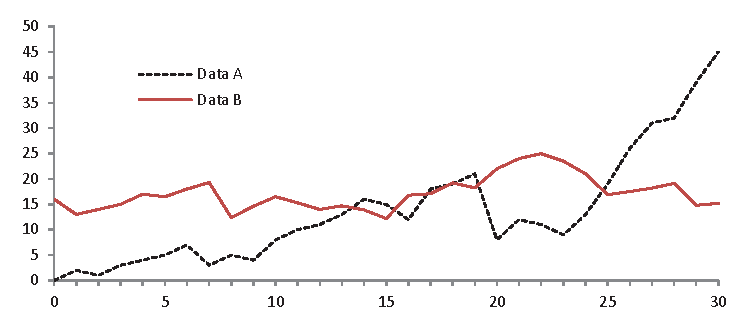
\includegraphics[width=\textwidth]{fig1.eps}
\caption{A figure caption is always placed below the illustration.
Please note that short captions are centered, while long ones are
justified by the macro package automatically.} \label{fig1}
\end{figure}

\begin{theorem}
This is a sample theorem. The run-in heading is set in bold, while
the following text appears in italics. Definitions, lemmas,
propositions, and corollaries are styled the same way.
\end{theorem}
%
% the environments 'definition', 'lemma', 'proposition', 'corollary',
% 'remark', and 'example' are defined in the LLNCS documentclass as well.
%
\begin{proof}
Proofs, examples, and remarks have the initial word in italics,
while the following text appears in normal font.
\end{proof}
For citations of references, we prefer the use of square brackets
and consecutive numbers. Citations using labels or the author/year
convention are also acceptable. The following bibliography provides
a sample reference list with entries for journal
articles~\cite{ref_article1}, an LNCS chapter~\cite{ref_lncs1}, a
book~\cite{ref_book1}, proceedings without editors~\cite{ref_proc1},
and a homepage~\cite{ref_url1}. Multiple citations are grouped
\cite{ref_article1,ref_lncs1,ref_book1},
\cite{ref_article1,ref_book1,ref_proc1,ref_url1}.
\section{Conclusions}
Conclusion
%
% ---- Bibliography ----
%
% BibTeX users should specify bibliography style 'splncs04'.
% References will then be sorted and formatted in the correct style.
%
\bibliographystyle{splncs04}
\bibliography{mybibliography}
%
\end{document}
